\newpage
\section{2019春}
\setcounter{yearcounter}{2019}

\subsection{弾性体と構造の力学(1)}
\spprob{
  図1のような等方均質な線形弾性体の円板が平面応力状態にあり、
  一様に分布する応力テンソルが次のようであったとする。
  以下の問いに答えよ。
  \begin{gather}
    [\grs]
    = \bmat{
      \grs_{x} & \tau_{xy} \\
      \tau_{xy} & \grs_{y}
    } = \bmat{
      -5 & -7\sqrt{3} \\
      -7\sqrt{3} & 9
    } \quad(\si{M Pa})
  \end{gather}

  % PIC
  % \begin{figure}[H]\centering
  %   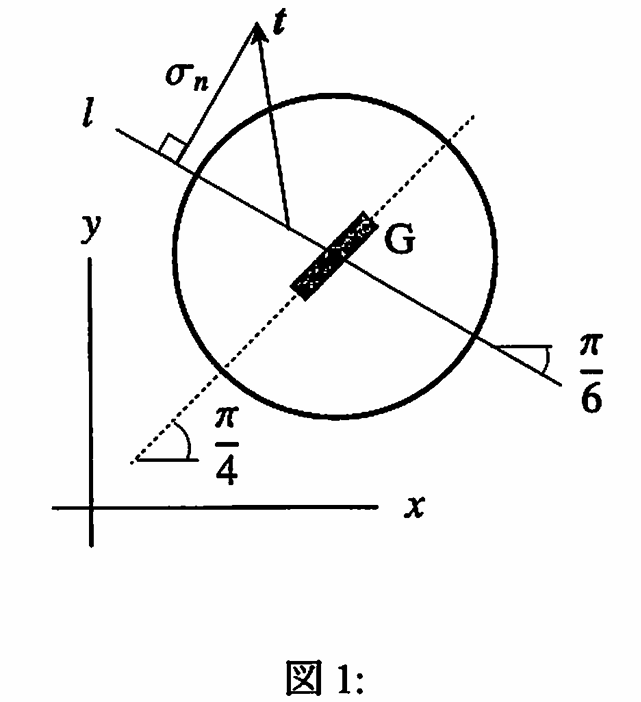
\includegraphics[width=.35\linewidth]{./src/fig/Specialized/S_2019_spring_01.png}
  % \end{figure}

  \begin{enumerate}[label=\arabic*.]
    \item 主応力$\grs_{1},\,\grs_{2}$とその主方向の単位ベクトル
    \dm{
      \bn_{1} = \Bmat{
        n_{1x} \\ n_{1y}
      },\,\bn_{1} = \Bmat{
        n_{2x} \\ n_{2y}
      }
    }を求めよ。
    \item $x$軸から時計回りに\dm{\frac{\pi}{6}}傾いた線$l$上に作用する
    表面力ベクトル$\bt$の$l$に垂直な成分$\grs_{n}$を求めよ。
    \item モール円を描いて(1)式の応力状態に対応する点を示せ。
    \item 材料のヤング率を$E=\SI{400}{MPa}$、ポアソン比を$\nu=0.25$とするとき、
    主ひずみ$\ve_{1},\,\ve_{2}$、および$x$軸から反時計回りに\dm{\frac{\pi}{4}}傾いたひずみゲージGが感知するひずみ$\ve_{\rm{G}}$を求めよ。
  \end{enumerate}
}

\subsection{弾性体と構造の力学(2)}
\spprob{
  \begin{enumerate}[label=\arabic*.]
    \item 図-1の単純梁ABに対して集中荷重$P$と等分布荷重$w$が作用するとき、C点の鉛直変位を求めよ。
    ただし、はりの曲げ耐性は$EI = \rm{const.}$とする。

    % PIC
    % \begin{figure}[H]\centering
    %   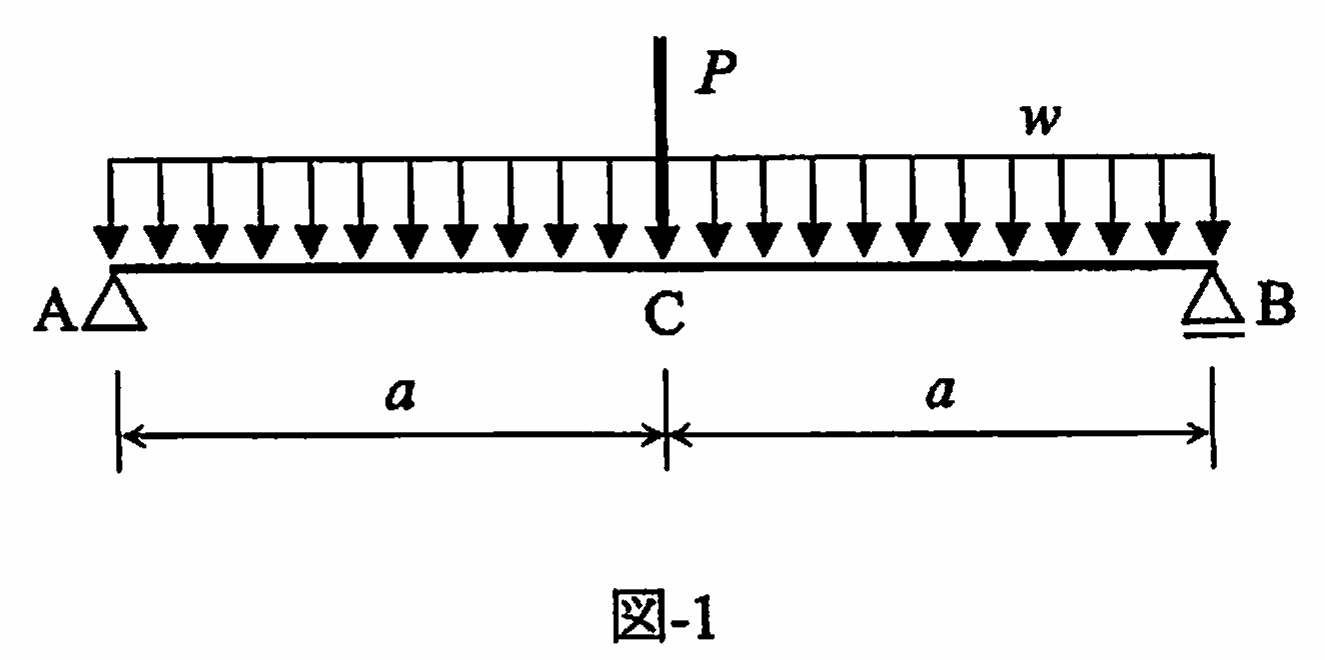
\includegraphics[width=.5\linewidth]{./src/fig/Specialized/S_2019_spring_02.png}
    % \end{figure}

    \item 図-2の片持ち梁OAに対して側方から静水圧荷重が作用するとき、以下の問いに答えよ。
    ただし、O点での静水圧は$w_{0}$であり、片持ち梁の曲げ剛性は$EI=\rm{const.}$とする。
    \begin{enumerate}[label=(\arabic*)]
      \item 図-2について、A点の水平変位を求めよ。
      \item 図-3に示すようにA点に両端ヒンジの水平部材ABを取り付けたとき、水平部材ABに作用する軸力を求めよ。
      ただし、水平部材ABの圧縮剛性は$E_{0}A_{0}=\rm{const.}$とし、座屈は生じないものとする。

      % PIC
      % \begin{figure}[H]\centering
      %   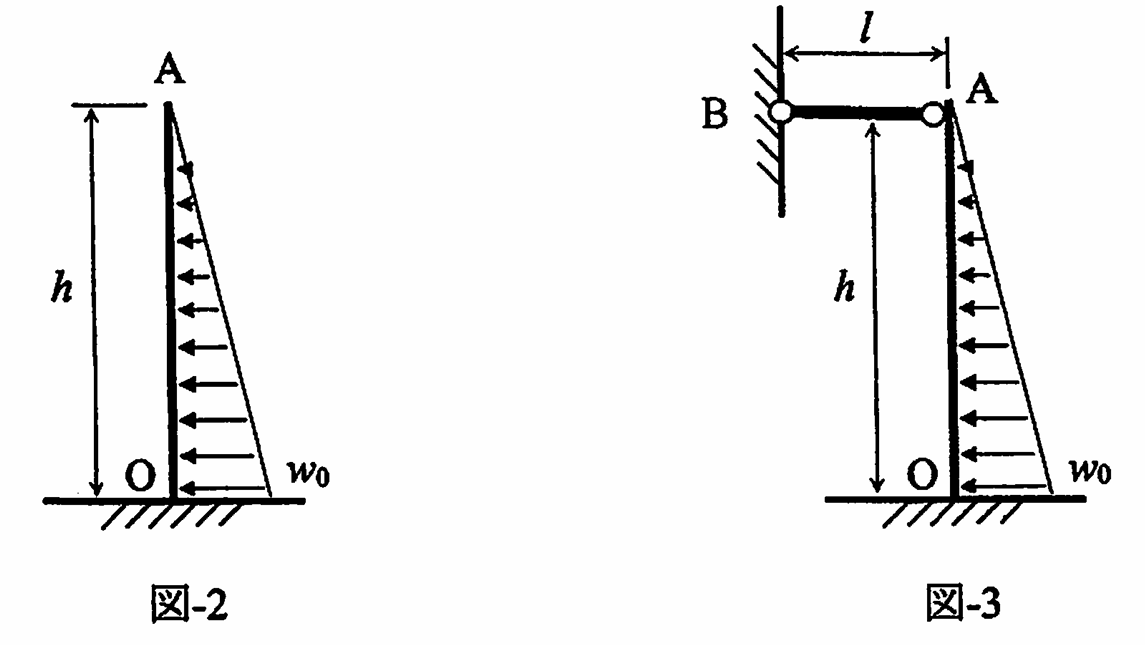
\includegraphics[width=.6\linewidth]{./src/fig/Specialized/S_2019_spring_03.png}
      % \end{figure}
    \end{enumerate}
  \end{enumerate}
}

\subsection{地盤とコンクリート(1)}
\spprob{
  \begin{enumerate}[label=\arabic*.]
    \item 粘性土に対して圧密非排水($\overline{\rm{CU}}$)三軸圧縮試験を行った。\\
    圧密応力$\grs'_{0}$を$\SI{100}{kPa},\,\SI{200}{kPa},\,\SI{300}{kPa}$として等方圧密を行った後、
    軸圧縮を行ったところ、それぞれ下表の状態に達したときに供試体が破壊した。
    この粘性土のせん断強さはモール・クーロンの破壊基準に従うものとし、以下の問に答えよ。

    なお、計算には以下の近似値を用いてよい
    \dm{\colon
      \sin30\deg = 0.50,\,
      \cos30\deg \approx 0.87,\,
      \sin32\deg \approx 0.53,\,
      \cos32\deg \approx 0.85,\,
      \sin34\deg \approx 0.56,\,
      \cos34\deg \approx 0.83,\,
      \sin36\deg \approx 0.59,\,
      \cos36\deg \approx 0.81
    }

    \begin{table}[H]
    \centering
    \begin{tabular}{lccc}
    \toprule
       & 試験1 & 試験2 & 試験3 \\
    \midrule
      圧密応力$\grs'_{0}$(\si{kPa}) & 100 & 200 & 300 \\
      破壊時の主応力差(軸差応力)$\grs_{\rm{d,max}}$(\si{kPa}) & 101.8 & 186.6 & 271.4 \\
      破壊時の過剰間隙水圧$\Delta u_{\rm{f}}$(\si{kPa}) & 70.9 & 133.3 & 195.7 \\
    \bottomrule
    \end{tabular}\end{table}

    \begin{enumerate}[label=(\arabic*)]
      \item 各試験での破壊時の最大有効主応力$\grs'_{\rm{1f}}$および最小有効主応力$\grs'_{\rm{3f}}$を求めよ。
      \item 次式で定義される$p'_{\rm{f}}$および$q_{\rm{f}}$を用いて、試験結果を$p'_{\rm{f}}\text{-}q_{\rm{f}}$平面上にプロットせよ。
      \begin{gather}
        p'_{\rm{f}} = \frac{\grs'_{\rm{1f}} + \grs'_{\rm{3f}}}{2} ,\,
        q_{\rm{f}} = \frac{\grs'_{\rm{1f}} - \grs'_{\rm{3f}}}{2}
      \end{gather}
      \item この粘性土の有効応力表示での粘着力$c'$と内部摩擦角$\grp'$を求めよ。
    \end{enumerate}
    \item 下図に示すような高さ\SI{10}{m}の擁壁に作用する土圧について、以下の問に答えよ。
    擁壁背後は水平で、背後地盤の土は均質で、その物性値は図中に示す通りである。
    ランキンの土圧理論により、主働土圧係数は$K_{\rm{a}}=(1-\sin\grp')/(1+\sin\grp')$と与えられる。
    また、水の単位体積重量は$\grg_{\rm{w}}=\SI{9.8}{kN/m^3}$とする。

    % PIC
    % \begin{figure}[H]\centering
    %   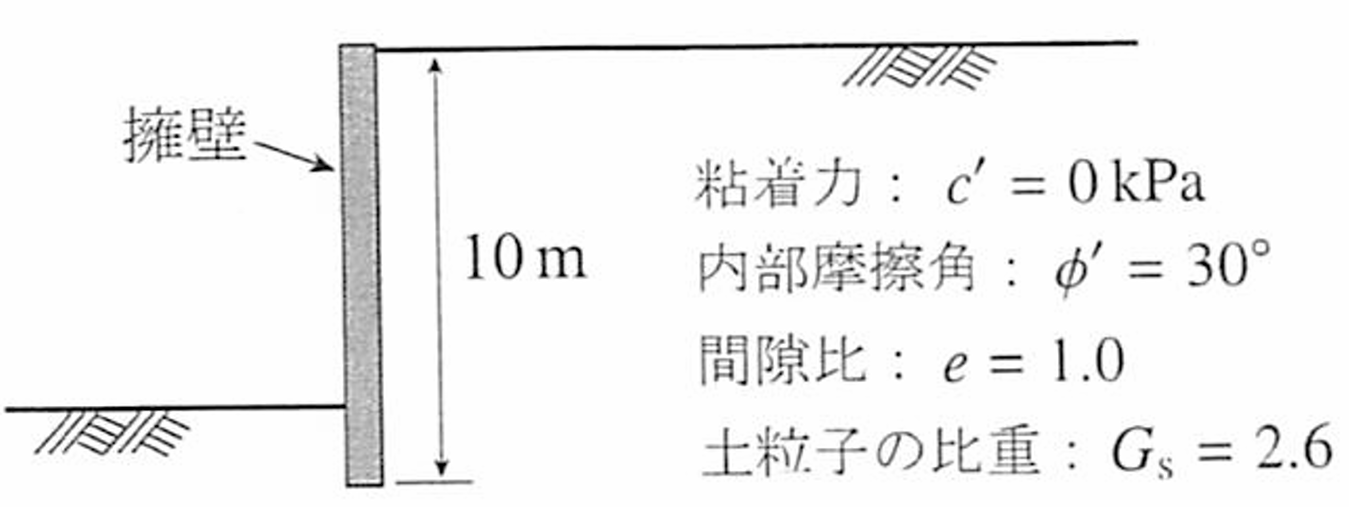
\includegraphics[width=.45\linewidth]{src/fig/Specialized/S_2019_spring_04.png}
    % \end{figure}

    \begin{enumerate}[label=(\arabic*)]
      \item 地下水位が背後地盤の地表面にあるとき、擁壁に作用する主働土圧の合力を求めよ。
      ただし、背後地盤の土の飽和単位体積重量は$\grg_{\rm{sat}}=\SI{17.64}{kN/m^3}$とする。
      \item その後、地下水位が擁壁下端よりも深い位置まで低下し、背後地盤の土の飽和度$S_{\rm{r}}$は$40\%$まで一様に低下した。
      このときの土の湿潤単位体積重量$\grg_{\rm{t}}$を求めよ。
      \item 全問(2)のとき、擁壁に作用する主働土圧の合力を求めよ。
    \end{enumerate}
  \end{enumerate}
}

\subsection{地盤とコンクリート(2)}
\spprob{
  \begin{enumerate}[label=\arabic*.]
    \item 図-1に示すように、長方形断面を有するコンクリート単純支持梁に、PC鋼材によってプレストレス力導入されるとともに、
    等分布の死荷重(自重)と活荷重が作用する場合について、以下の問いに答えよ。
    なお、梁は弾性体と仮定してよい。
    \begin{enumerate}[label=(\arabic*)]
      \item 梁に、①プレストレス力のみが作用した場合、②さらに等分布の死荷重と活荷重が作用した場合、
      の2ケースについて、支間中央の断面に生じる応力分布形状を図示せよ。
      \item 導入するプレストレス力の大きさによって、断面の応力分布形状がどのように変化するかを図示せよ。
      \item (2)で求めた応力分布を用いて、鉄筋コンクリート梁とプレストレストコンクリート梁の違いを説明せよ。
    \end{enumerate}

    % PIC
    % \begin{figure}[H]\centering
    %   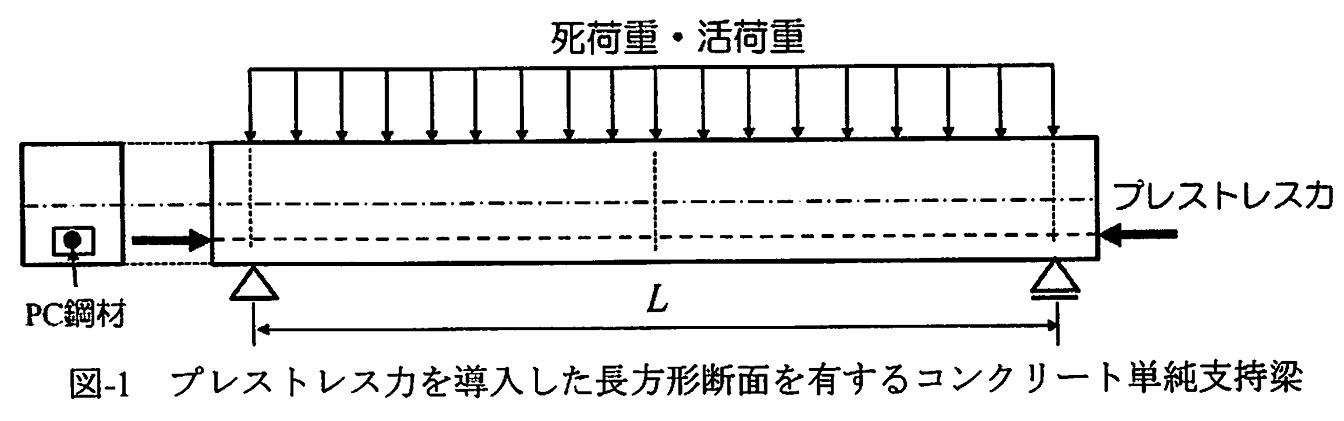
\includegraphics[width=.6\linewidth]{./src/fig/Specialized/S_2019_spring_05.png}
    % \end{figure}

    \item 鉄筋コンクリートの中性化による劣化メカニズムを説明せよ。
    さらに、劣化進展抑制のための対策方法を1つあげ、抑制メカニズムについて説明せよ。
    \item 次のコンクリート工学に関する専門用語を説明せよ。
    \begin{enumerate}[label=(\arabic*)]
      \item 限界状態設計法
      \item レイタンス
      \item AEコンクリート
      \item コンクリート部材に用いる連続繊維補強材
    \end{enumerate}
  \end{enumerate}
}
